%META {"question":"Trên hình có ba tia Ox, Oy, Oz chung gốc O (Ox và Oy đối nhau). Có tất cả bao nhiêu tia chung gốc O?","options":["3 tia","2 tia","6 tia","1 tia"],"answer":0,"note":"Mỗi tia được xác định bởi gốc O và một hướng: Ox, Oy, Oz là 3 tia khác nhau. Ox và Oy đối nhau nhưng vẫn là hai tia riêng biệt."}
\documentclass[border=5pt]{standalone}
\usepackage{tkz-euclide}
% Màu dùng chung cho toàn bộ hình vẽ (ảnh stack với nền tối của web)
\definecolor{tminc}{RGB}{226,232,240}   % chữ + nét chính
\definecolor{tmblue}{RGB}{0,210,255}    % nhấn neon xanh
\definecolor{tmpink}{RGB}{255,0,200}    % nhấn neon hồng
\definecolor{tmgreen}{RGB}{0,255,136}   % nhấn neon xanh lá
\color{tminc}

\begin{document}
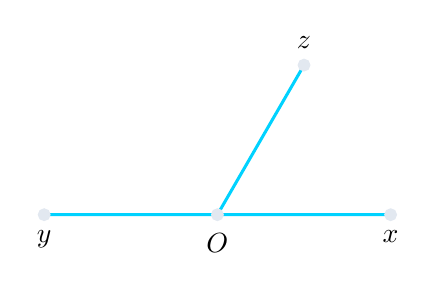
\begin{tikzpicture}[line width=1.1pt]
  \coordinate (Y) at (-0.4,0);
  \coordinate (O) at (1.8,0);
  \coordinate (X) at (4,0);
  \coordinate (Z) at (2.9,1.9);
  \draw[tmblue] (O) -- (X) (O) -- (Y) (O) -- (Z);
  \tkzDrawPoints[size=3.5,color=tminc,fill=tminc](O,X,Y,Z)
  \tkzLabelPoint[below=3pt](O){$O$}
  \tkzLabelPoint[below=2pt](X){$x$}
  \tkzLabelPoint[below=2pt](Y){$y$}
  \tkzLabelPoint[above=2pt](Z){$z$}
\end{tikzpicture}
\end{document}
